\documentclass[journal,12pt,onecolumn]{IEEEtran}
\usepackage[utf8]{inputenc}   % Codificación de entrada
\usepackage[T1]{fontenc}      % Codificación de fuente
\usepackage[spanish,es-tabla]{babel}   % Idioma español
\usepackage{lmodern}          % Fuente moderna
\usepackage{amsmath, amssymb} % Matemáticas y símbolos
\usepackage{graphicx} 		  % Gráficos e imágenes
\graphicspath{{img/}{tablas/}{portada/}}  % Las imágenes se buscarán en la carpeta "img"
\usepackage{longtable}      % Para tablas que se extienden en varias páginas
\usepackage{tabularx}	% Tablas avanzadas
\usepackage{threeparttable}
\usepackage{hyperref}	% Hipervínculos

%-------------------------------------------
% Otros paquetes útiles (personaliza según tus necesidades)
%-------------------------------------------
\usepackage{caption}
\usepackage{subcaption}
\usepackage{xcolor}
\usepackage{setspace}

%-------------------------------------------
% Comandos personalizados
\renewcommand{\listtablename}{Índice de tablas}
\renewcommand{\appendixname}{Anexos}
\definecolor{colorreferences}{RGB}{48,134,3}

% Metadatos del PDF
\hypersetup{
	unicode=true,
	hidelinks,
	colorlinks=true,       % false: boxed links; true: colored links
	linkcolor=black,          % color of internal links (change box color with linkbordercolor)
	citecolor=colorreferences,        % color of links to bibliography
	filecolor=magenta,      % color of file links
	urlcolor=blue,           % color of external links
	linkbordercolor={0 0 0}
}
%-------------------------------------------
% Inicio del documento
%-------------------------------------------
\begin{document}

% Aquí se encuentra el archivo con la portada
\begin{titlepage}
	\centering
	%-------------------------------------------
	% Logos en una tabla: izquierda, centro y derecha
	\begin{tabular}{@{}p{0.3\textwidth} p{0.3\textwidth} p{0.3\textwidth}@{}}
		
\includegraphics[height=2cm]{tecnm} & 
		\centering 
\includegraphics[height=1.5cm]{SEP} & 
		\raggedleft 
\includegraphics[height=2cm]{ith.jpg} \\
	\end{tabular}
	
	\vspace{2em}
	
	\noindent
	%-------------------------------------------
	%	Información institucional y académica (esquina superior izquierda)
	\begin{minipage}[t]{0.6\textwidth}
		\raggedright
		\small \textbf{%
			Instituto Tecnológico de Hermosillo\\
			Materia: Robótica\\
			Profesor: Medina Gil Lamadrid, Jesús Iván%
		}
	\end{minipage}%
	\hfill
	%	fecha actual (esquina superior derecha), en letras pequeñas y en negrita.
	\begin{minipage}[t]{0.3\textwidth}
		\raggedleft
		\small \textbf{\today}
	\end{minipage}
	
	\vspace{2em}
	
	%-----------------------------------------
	% Unidad y Título de la tarea en letras grandes y en negrita
%	{\large \textbf{Unidad Final}}\\
	{\Huge \textbf{Reporte final del Robot}}
		
	\vspace{1em}
	
	%---------------------------------------
	% Tabla con la información del equipo
	%---------------------------------------
	% Encabezado del equipo
	\begin{center}
		{\Large \textbf{Equipo N}}
		
		{\small \textbf{https://github.com/DueñoDelRepositorio/Robotica.git}}
	\end{center}
	
	\vspace{1em}
	
	% Tabla de integrantes:
	% Cada fila contiene: foto (columna izquierda) y datos del integrante (columna derecha)
	\begin{center}
		\begin{tabular}{c c}
			\begin{tabular}{c}
				
\includegraphics[height=3cm]{perfil1.jpg} \\
				\textbf{Apellido1},\\ Nombre1 \\ \texttt{correo1@ejemplo.com} \\ Teléfono: (opcional)
			\end{tabular} &
			\begin{tabular}{c}
				
\includegraphics[height=3cm]{perfil2.jpg} \\
				\textbf{Apellido2,}\\ Nombre2 \\ \texttt{correo2@ejemplo.com} \\ Teléfono: (opcional)
			\end{tabular} \\ \vspace{2em}
			\begin{tabular}{c}
				
\includegraphics[height=3cm]{perfil3.jpg} \\
				\textbf{Apellido3,}\\ Nombre3 \\ \texttt{correo3@ejemplo.com} \\ Teléfono: (opcional)
			\end{tabular} &
			\begin{tabular}{c}
				
\includegraphics[height=3cm]{perfil4.jpg} \\
				\textbf{Apellido4,}\\ Nombre4 \\ \texttt{correo4@ejemplo.com} \\ Teléfono: (opcional)
			\end{tabular}
		\end{tabular}
	\end{center}

\end{titlepage}

%	Es innecesario poner el índice porque ya aparece en los marcadores del PDF
%\tableofcontents

% Ejemplo de inclusión de una sección (por ejemplo, "introduccion.tex" debe estar en la carpeta "secciones" y se recomienda no usar carácteres especiales (tilde) o espacios)
\section{Introducción}
\LaTeX es una herramienta poderosa para la creación de documentos técnicos y científicos, permitiendo la generación de contenido con alta calidad tipográfica. En este documento se han explorado diferentes aspectos fundamentales para la creación de reportes en \LaTeX, incluyendo la inserción de imágenes, la organización de tablas y la formulación de ecuaciones matemáticas.

Algo que se puede dar a notar es que las secciones tienen nombres un pcoo diferentes a los que están acostumbrados. Les doy libertad para usar nombres libres o usar nombres clásicos, como marco teórico. También pueden usar una sección llamada marco teórico y subsecciones más específicas como puse en la \autoref{sec:conclusion}: Conclusión.

Aun hay muchas cosas que no se abarcaron en este documento, pero pueden preguntarle a chatGPT, a Deepseek o simplemente googlearlo. 

\section{Imágenes}
En \LaTeX, las imágenes se pueden incluir utilizando el paquete \texttt{graphicx}. 
Para añadir una imagen en texstudio, es posible arrastrarla directamente en el editor, lo que obtendrá como resultado lo mostrado en la \autoref{fig:insertarimagen}.

\begin{figure}[h]
	\centering
	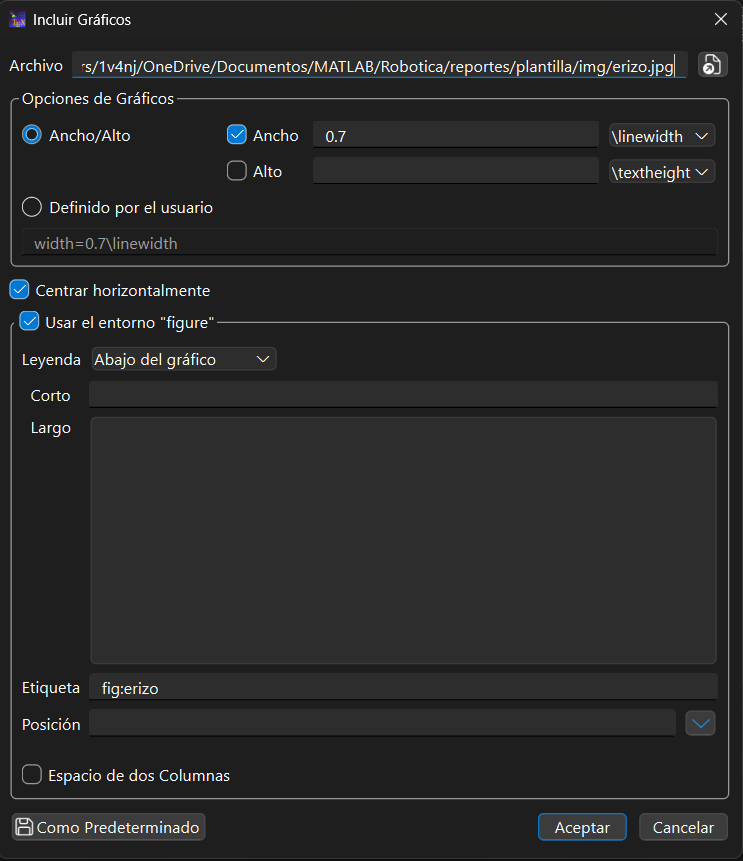
\includegraphics[width=0.7\linewidth]{img/insertarImagen}
	\caption{Opciones al insertar una imagen}
	\label{fig:insertarimagen}
\end{figure}

Algunas opciones clave incluyen:

\begin{itemize}
	\item \textbf{Tamaño de la imagen}: Se puede definir un ancho o alto relativo a la caja de texto o se puede usar un tamaño en pixeles (px), centímetros (cm) o el ancho de la letra M (em).
	\item \textbf{Centrado}: Se puede marcar la opción para que la imagen aparezca centrada automáticamente.
	\item \textbf{Uso del entorno `figure'}: Permite que la imagen tenga una numeración automática y pueda referenciarse en el texto con \texttt{\textbackslash ref\{\}} o \texttt{\textbackslash autoref\{\}}.
	\item \textbf{Posicionamiento (`h`, `t`, `b`, `p`)}: Al presionar la flecha de la derecha, podemos añadir las opciones que determinan la posición de la imagen en el documento, como después del texto o arriba de la página, etc. Si igual vamos a referenciar las figuras, es innecesario que estén exactamente donde fueron mencionadas ya que eso deja muchos espacios en blanco.
	\item \textbf{Leyenda Largo}: permite poner una descripción de la imagen en el lugar que elegimos (debería de estar debajo).
	\item \textbf{Etiqueta}: nos servirá para referenciarla. 
\end{itemize}

Para usar dos imágenes como en \autoref{fig:mascotas}, se utilizó \texttt{subfloat}.
% Dos imágenes de mascotas
\begin{figure}[h]
	\centering
	\subfloat[Perro]{%
		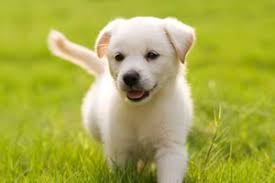
\includegraphics[width=0.4\textwidth]{perro.jpg}%
		\label{fig:perro}
	}
	\hfill
	\subfloat[Gato]{%
		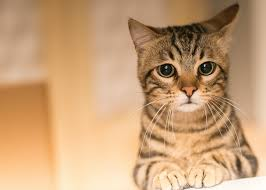
\includegraphics[width=0.4\textwidth]{gato.jpg}%
		\label{fig:gato}
	}
	\caption{Imagen de dos mascotas}
	\label{fig:mascotas}
\end{figure}



\section{Ecuaciones}
Para realizar ecuaciones, se pueden ayudar mucho de ChatGPT (Como copiar una imagen y que lea la ecuación para dártela en formato \LaTeX) y de que MATLAB, word y algunas páginas te permiten copiar ecuaciones en formato \LaTeX. El modelo en espacio de estados de un robot de dos grados de libertad, el cual se puede ver en el Capítulo 5: Dinámica del Robot en \cite{barrientos2007fundamentos} se expresa como

\begin{equation}
	\label{eq:spaceStateRobot}
	\begin{bmatrix}
		\dot{q} \\
		\ddot{q}
	\end{bmatrix} =
	\begin{bmatrix}
		0 & I \\
		M^{-1}(-C - G)
	\end{bmatrix}
	\begin{bmatrix}
		q \\
		\dot{q}
	\end{bmatrix} +
	\begin{bmatrix}
		0 \\
		M^{-1} B
	\end{bmatrix} u,
\end{equation}
donde:
\begin{itemize}
	\item \( q \) es el vector de posiciones articulares del robot.
	\item \( \dot{q} \) y \( \ddot{q} \) son las velocidades y aceleraciones articulares.
	\item \( M \) es la matriz de inercia.
	\item \( C \) representa las fuerzas centrífugas y de Coriolis.
	\item \( G \) es el vector de fuerzas gravitacionales.
	\item \( B \) es la matriz de entrada de los torques.
	\item \( u \) es el vector de torques aplicados a las articulaciones.
\end{itemize}

Cabe destacar que en \eqref{eq:spaceStateRobot}, la ecuación se referencia después de haberla nombrado y forma parte de la oración, por lo que debe llevar puntos o comas. También al referenciar, debe de estar entre paréntesis con \texttt{eqref}.
\section{Conclusión} \label{sec:conclusion}
Los sensores internos y externos son fundamentales en la recopilación de datos y el monitoreo de sistemas, diferenciándose por su ubicación y las variables que miden. Los sensores internos se encuentran dentro de un dispositivo o sistema, supervisando condiciones internas como temperatura, presión o voltaje, y son clave para asegurar el correcto funcionamiento y estabilidad de equipos, como motores o baterías. Por otro lado, los sensores externos están ubicados fuera del sistema y se utilizan para detectar estímulos en el entorno, como proximidad, movimiento o gases, y son esenciales en aplicaciones como seguridad, monitoreo ambiental o control de procesos industriales. Ambos tipos trabajan en conjunto para crear sistemas más eficientes, inteligentes y seguros, mejorando la interacción con el entorno y optimizando el rendimiento.


%-------------------------------------------
% Bibliografía
%-------------------------------------------
\bibliographystyle{IEEEtran}  % Estilo de bibliografía IEEE
% La bibliografía se tomará del archivo "fuentes.bib"
\bibliography{fuentes}
	
\end{document}
